\documentclass[landscape,a3paper,fontscale=0.75,margin=0.4cm]{baposter}

\usepackage[ansinew]{inputenc} 
\usepackage{graphicx}
\usepackage{amsmath}
\usepackage{amssymb}
\usepackage{relsize}
\graphicspath{{images/}}

\newcommand{\textsup}[1]{\raisebox{.4em}{\footnotesize #1}}


%%% Color Definitions %%%%%%%%%%%%%%%%%%%%%%%%%%%%%%%%%%%%%%%%%%%%%%%%%%%%%%%%%

\definecolor{bordercol}{RGB}{204,204,204}
\definecolor{headercol1}{RGB}{198,219,239}
\definecolor{headercol2}{RGB}{222,235,247}
\definecolor{headerfontcol}{RGB}{0,0,0}
\definecolor{boxcolor}{RGB}{255,255,255}
\definecolor{BgColor1}{RGB}{247,251,255}  % Colorbrewer's ''Blues''
\definecolor{BgColor2}{RGB}{158,202,255}

%% colours in genome partition; colorbrewer2.org, PRGn (purple-white-green)
%% purple -- RGB: 123,50,148; HSL: 202,126,99; #7C3294
%% green -- RGB: 0,136,55;  HSL: 102,255,68; #008836
%% de-saturated purple -- RGB:  99,99,99;  HSL: 202,0,99;  #636363

%\renewcommand{\familydefault}{\aupassata}  % This command changes the default font to AU Passata


\begin{document}
\typeout{Poster rendering started}
\begin{poster}{
    %%%%%%%%%%%%%%%%%%%%%%%%%%%%%%%%%
    %% Options
    grid=false,
    columns=3,
    colspacing=1.2em,
    linewidth=2pt,
    logosetup=topbar,
    headerheight=0.18\textheight, % Height of header-bar, multiplied by some magic constant.
    %%%%%%%%%%%%%%%%%%%%%%%%%%%%%%%%%
    %% Background options
    bgColorOne=BgColor1,
    bgColorTwo=BgColor2,
    background=none, %shadeTB,
    borderColor=bordercol,
    %%%%%%%%%%%%%%%%%%%%%%%%%%%%%%%%%
    %% Format of text header
    headerColorOne=headercol1,
    headerColorTwo=BgColor1,
    headershade=shadeLR,
    headerFontColor=headerfontcol,
    headerborder=none,
    headershape=roundedleft,
    headerfont=\Large\sf\bf, %% Other fun options \sffamily\bfseries or %\Large\sf\bf,
    %%%%%%%%%%%%%%%%%%%%%%%%%%%%%%%%%
    %% Format of textbox
    textfont=\rmfamily, %\usefont{T1}{aupassata}{m}{n}, %\sffamily, %\rmfamily % sans-serif (sffamily) or roman (rmfamily)
    textborder=none,
    boxColorOne=boxcolor,
    %boxshade=none,
    boxpadding=1em
}
%%% Top logo, stretches entire width of page %%%%%%%%%%%%%%%%%%%%%%%%%%%%%%%%%%
{
  \hspace{-1.5em}
  
\includegraphics[width=\textwidth,keepaspectratio=true]{qgg-a3-portrait}  
}
%%% Title %%%%%%%%%%%%%%%%%%%%%%%%%%%%%%%%%%%%%%%%%%%%%%%%%%%%%%%%%%%%%%%%%%%%%
{ 
  Genetic partitioning of the genome
}
%%% Authors %%%%%%%%%%%%%%%%%%%%%%%%%%%%%%%%%%%%%%%%%%%%%%%%%%%%%%%%%%%%%%%%%%%
{
  Stefan McKinnon H{\o}j-Edwards\textsup{1}
  
  \small \textsup{1}Centre for Quantitative Genetics and Genomics, Department of Molecular Biology and Genetics, Aarhus University, Denmark.
}
{
  \includegraphics[width=0.1\textwidth,keepaspectratio=true]{{datamatrix.png}}  
}




%%%%%%%%%%%%%%%%%%%%%%%%%%%%%%%%%%%%%%%%%%%%%%%%%%%%%%%%%%%%%%%%%%%%%%%%%%%%%%%
%% Poster contents
%%%%%%%%%%%%%%%%%%%%%%%%%%%%%%%%%%%%%%%%%%%%%%%%%%%%%%%%%%%%%%%%%%%%%%%%%%%%%%%

%%%%%%%%%%%%%%%%%%%%%%%%%%%%%%%%%%%%%%%%%%%
%% Problem
%%%%%%%%%%%%%%%%%%%%%%%%%%%%%%%%%%%%%%%%%%%
\begin{posterbox}[name=problem,column=0,row=0]{Problem}
  Is is possible to partition a genome's markers into those that have a high marker effect vs. those with low marker effect.
  \vspace{4em}
\end{posterbox}  

\begin{posterbox}[name=genome,column=0,below=problem]{Genomic partitioning}
  \begin{center}
    \vspace{0.12in}
  	\includegraphics[page=3,height=1.37in,keepaspectratio=true]{figures}
  	\vspace{0.312in}
  	
  	\itshape{By including using any kind of external information, e.g.\ KEGG pathways, we can partition the genome into two sets, purple ($\mathcal{S}$) and green ($\neg\mathcal{S}$).}
  \end{center}

\end{posterbox}

\begin{posterbox}[name=conclusion,column=1,span=2,row=0]{Conclusion}
    \begin{itemize}
     \item Splitting markers into those with higher or low marker effect improves model fitting.
     \item Something to do with the infinitesimal model.
     \item Generated results here indicate it also improves prediction of new genotypes.
     \item Excel charts are to graphical design what bricks are to poetry.
    \end{itemize}
\end{posterbox}

%\begin{posterbox}[name=ghost1,column=1,below=conclusion,boxheaderheight=0em,boxshade=none]{}
%    \vspace{0.5em}
%\end{posterbox}

%%%%%%%%%%%%%%%%%%%%%%%%%%%%%%%%%%%%%%%%%%%
%% Acknowledgements
%%%%%%%%%%%%%%%%%%%%%%%%%%%%%%%%%%%%%%%%%%%
\begin{posterbox}[name=ack,column=2,below=genome]{Acknowledgements}
   Thanks to cras sit amet tortor ante, id porttitor velit. Proin et dictum elit. Maecenas tempor tristique ullamcorper. 
   Maecenas nulla turpis, mollis nec vulputate sit amet, faucibus sed magna.
   
   \vspace{1em}
   %\begin{wrapfigure}{l}[2]{0pt} % requires wrapfig package
   %\end{wrapfigure}
	 
\begin{flushright}

	 \begin{minipage}[c]{0.7\linewidth}
	 	 \vspace{0.2in}
		 \begin{flushright}
		 	 \footnotesize{ 
		 	   \hfill \texttt{stefan.hoj-edwards@agrsci.dk}
		 	   \newline
  	 	 	 \texttt{http://iysik.com/research/conference/icqg4} 
  	 	 }
  	 \end{flushright}   	 
 	 \end{minipage}
 	 \hspace{0.1em}
   \begin{minipage}[c]{0.15\linewidth}
		  
\includegraphics[width=0.5in,height=0.5in,trim=0.2in 0.2in 0.2in 0.2in,clip=true]{datamatrix.png}    
	 \end{minipage} 	 

\end{flushright}
   
\end{posterbox}

%%%%%%%%%%%%%%%%%%%%%%%%%%%%%%%%%%%%%%%%%%%
%% References
%%%%%%%%%%%%%%%%%%%%%%%%%%%%%%%%%%%%%%%%%%%
\begin{posterbox}[name=ref,column=0,below=genome]{References} 
  \footnotesize\par\begingroup
    \leftskip=0.5in \parindent=-\leftskip
    Albert, Leonard. ``Gnomonology: Joyce's `The Sisters'.'' \textit{James Joyce Quarterly} 27.2 (1990): 355--364. PDF.

    Aristotle. \textit{The Poetics}. Trans. W. Hamilton Frye. Cambridge: Harvard UP, 1927. Print. Loeb Classical Library 199, Aristotle 23. 
    
    Guererro, Frank. \emph{Giraffes in the Wild.} Philadelphia: Philadelphia Publishing Inc, 2002.
  \par\endgroup
\end{posterbox}


%%%%%%%%%%%%%%%%%%%%%%%%%%%%%%%%%%%%%%%%%%%
%% Middle graphic
%%%%%%%%%%%%%%%%%%%%%%%%%%%%%%%%%%%%%%%%%%%
\begin{posterbox}[name=fig1,column=1,below=problem]{Explained genetic variance}
  \begin{center}
        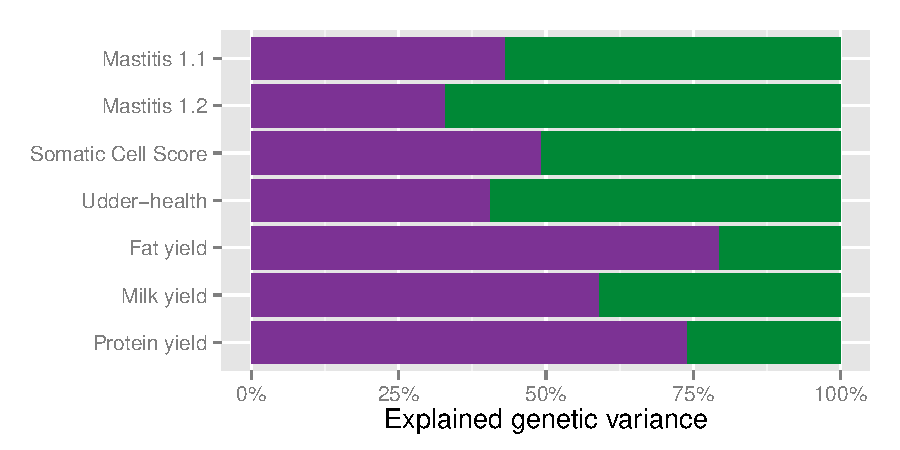
\includegraphics[scale=0.598,page=1]{figures} 
        
        \itshape{Amount of genetic variance explained by markers in purple and green areas of the genome for seven different phenotypic traits.}
  \end{center}
\end{posterbox}

%%%%%%%%%%%%%%%%%%%%%%%%%%%%%%%%%%%%%%%%%%%
%% Right graphic
%%%%%%%%%%%%%%%%%%%%%%%%%%%%%%%%%%%%%%%%%%%
\begin{posterbox}[name=fig2,column=2,below=problem]{Prediction ability}
  \begin{center}
        \includegraphics[scale=0.599,page=2]{figures} 
        
        \itshape{Comparison of prediction reliabilities for no partitioning, partitioning by all genes and by a selected partitioning for seven phenotypic traits.}
  \end{center}  
\end{posterbox}

%%%%%%%%%%%%%%%%%%%%%%%%%%%%%%%%%%%%%%%%%%%
%% Model
%%%%%%%%%%%%%%%%%%%%%%%%%%%%%%%%%%%%%%%%%%%
\begin{posterbox}[name=model,column=1,below=genome]{Model}
   \begin{equation*}
     \mathbf{y} = \mu + \mathbf{Z}_\mathcal{S} \mathbf{b}_\mathcal{S} + \mathbf{Z}_{\neg\mathcal{S}} \mathbf{b}_{\neg\mathcal{S}} + \mathbf{e}
   \end{equation*}
    where $\mathbf{y}$ is a vector of phenotypes, $\mathbf{Z}_\mathcal{S}$ a marker-incidence matrix for the markers in set $\mathcal{S}$,
    $\mathbf{b}_\mathcal{S}$ marker effects for ditto markers, $\neg \mathcal{S}$ indicates markers \emph{not} belonging to set $\mathcal{S}$ 
    and $\mathbf{e}$ model residuals.
    
    \vspace{0.5em}
    Variance components for $\mathbf{b}_\mathcal{S}$, $\mathbf{b}_{\neg\mathcal{S}}$ and $\mathbf{e}$ were estimated using the AI-REML algorithm in the software DMU.
\end{posterbox}

\begin{posterbox}[name=aulogo,column=0,above=bottom,boxheaderheight=0em,boxshade=none]{}
  
\includegraphics[scale=1]{au-mbg-en-au-blue}  %% If logo is defined for A4, scaling is for A3 141%, A2 200%, A1 283%, A0 400%
\end{posterbox}

\end{poster}
\end{document}